\documentclass[12pt,a4paper]{article}

% ---------- Paquetes ----------
\usepackage[utf8]{inputenc}
\usepackage[T1]{fontenc}
\usepackage{mathptmx} % Times New Roman
\usepackage[margin=2.5cm]{geometry}
\usepackage{tikz}
\usetikzlibrary{arrows.meta,positioning,shapes.multipart,shapes.geometric,calc}
\usepackage{booktabs}
\usepackage{longtable}
\usepackage{array}
\usepackage{enumitem}
\usepackage{titlesec}
\usepackage{hyperref}
\hypersetup{colorlinks=false, pdfborder={0 0 0}}

\titleformat{\section}{\normalfont\bfseries\large}{P\thesection.}{0.4em}{}
\renewcommand{\thesection}{\arabic{section}}

\setlength{\parindent}{0pt}
\setlength{\parskip}{0.6em}

\title{\textbf{Prueba Práctica --- Unidad IV \\ Sistema de Gestión de Pedidos}}
\author{}
\date{}

\begin{document}

\maketitle
\vspace{-2em}

% =====================================================
\section{Modelo de datos --- Diagrama de clases UML}
% =====================================================

El dominio establece cuatro clases principales:

\begin{itemize}[nosep]
    \item Cliente
    \item Pedido
    \item LíneaPedido
    \item Producto
\end{itemize}

Un cliente puede realizar cero o más pedidos; cada pedido tiene una o más líneas; cada línea referencia un producto.

\subsection*{Diagrama}

\begin{center}
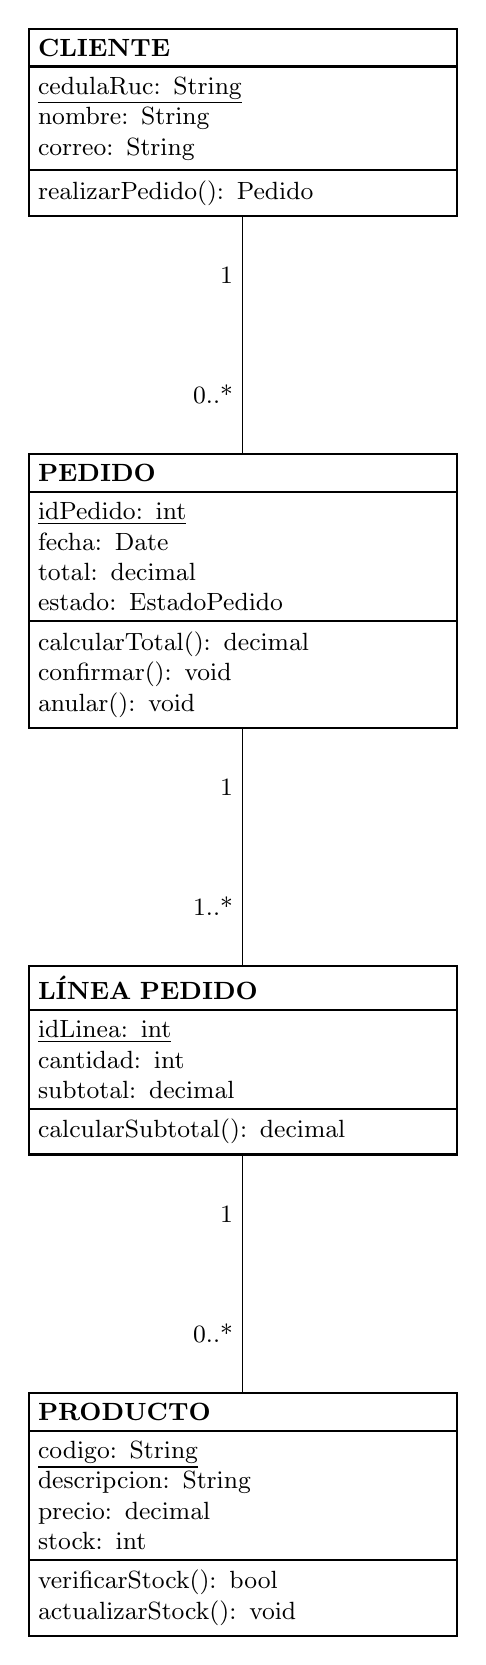
\begin{tikzpicture}[
    class/.style={rectangle split, rectangle split parts=3, draw=black, thick,
                  rectangle split part align={center,left,left},
                  text width=5.2cm, font=\small},
    every node/.style={font=\small}
]

\node[class] (cliente) {
    \textbf{CLIENTE}
    \nodepart{second} \underline{cedulaRuc: String} \\ nombre: String \\ correo: String
    \nodepart{third} realizarPedido(): Pedido
};

\node[class, below=3cm of cliente] (pedido) {
    \textbf{PEDIDO}
    \nodepart{second} \underline{idPedido: int} \\ fecha: Date \\ total: decimal \\ estado: EstadoPedido
    \nodepart{third} calcularTotal(): decimal \\ confirmar(): void \\ anular(): void
};

\node[class, below=3cm of pedido] (linea) {
    \textbf{LÍNEA PEDIDO}
    \nodepart{second} \underline{idLinea: int} \\ cantidad: int \\ subtotal: decimal
    \nodepart{third} calcularSubtotal(): decimal
};

\node[class, below=3cm of linea] (producto) {
    \textbf{PRODUCTO}
    \nodepart{second} \underline{codigo: String} \\ descripcion: String \\ precio: decimal \\ stock: int
    \nodepart{third} verificarStock(): bool \\ actualizarStock(): void
};

\draw[-] (cliente) -- (pedido)
    node[midway, left, xshift=-2pt] {}
    node[near start, left] {1}
    node[near end, left] {0..*};

\draw[-] (pedido) -- (linea)
    node[near start, left] {1}
    node[near end, left] {1..*};

\draw[-] (linea) -- (producto)
    node[near start, left] {1}
    node[near end, left] {0..*};

\end{tikzpicture}
\end{center}

\subsection*{Multiplicidades}

\begin{center}
\begin{tabular}{ll}
\toprule
\textbf{Asociación} & \textbf{Multiplicidad} \\
\midrule
Cliente $\rightarrow$ Pedido & 1 $\rightarrow$ 0..* \\
Pedido $\rightarrow$ Cliente & 1 \\
Pedido $\rightarrow$ LíneaPedido & 1 $\rightarrow$ 1..* \\
LíneaPedido $\rightarrow$ Pedido & 1 \\
LíneaPedido $\rightarrow$ Producto & 1 \\
Producto $\rightarrow$ LíneaPedido & 0..* \\
\bottomrule
\end{tabular}
\end{center}

Los identificadores están marcados con subrayado, cumpliendo la indicación de subrayarlos o marcarlos. La prueba exige atributos tipados, operaciones y multiplicidades.

% =====================================================
\section{Modelo funcional --- Registrador pedido}
% =====================================================

El proceso debe tener:

\begin{enumerate}[nosep]
    \item Inicio.
    \item Registro del pedido.
    \item Verificación del stock.
    \item Decisión.
    \begin{itemize}[nosep]
        \item Si existe stock $\rightarrow$ confirmar pedido.
        \item Si no existe $\rightarrow$ notificación faltante.
    \end{itemize}
    \item Convergencia.
    \item Fin.
\end{enumerate}

Esto corresponde exactamente a lo solicitado en P2.

\subsection*{Diagrama de actividades}

\begin{center}
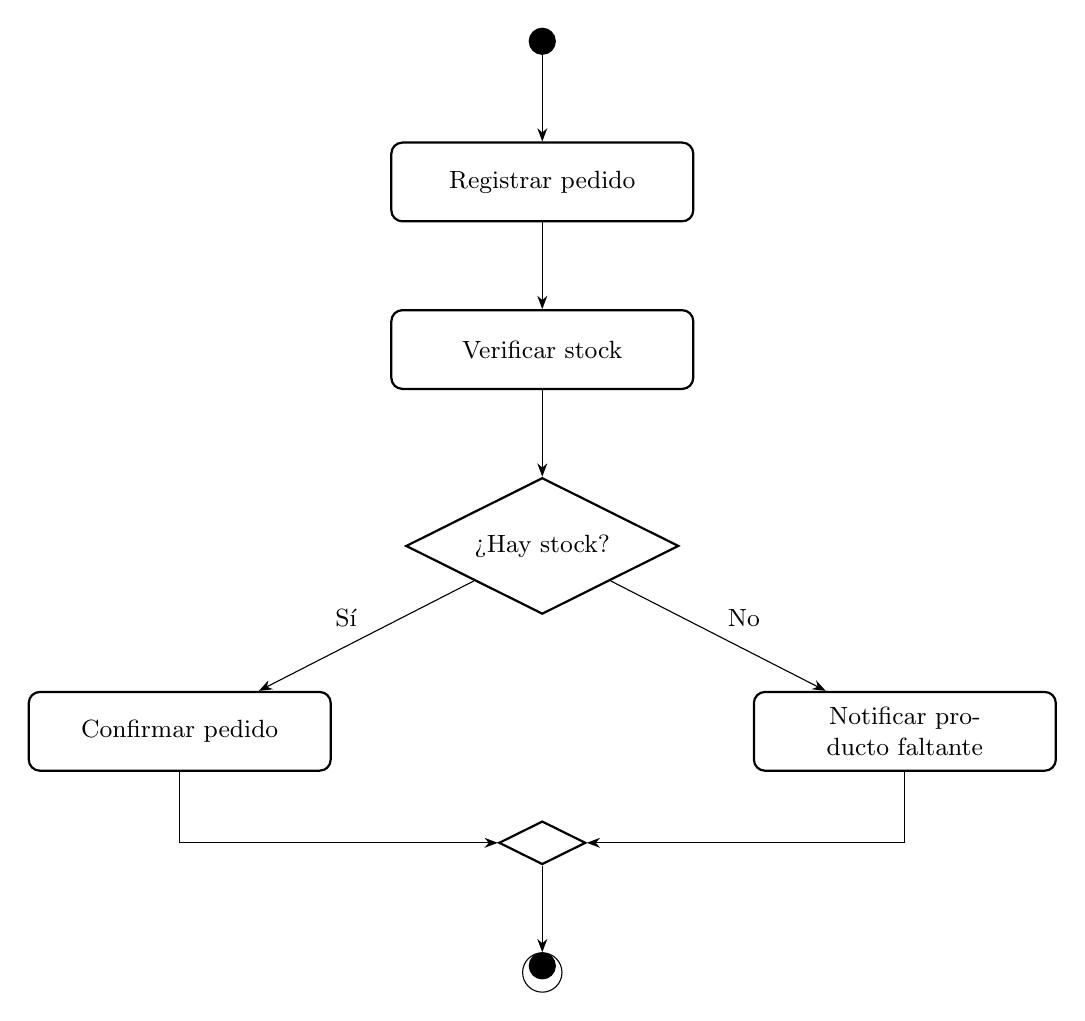
\begin{tikzpicture}[
    node distance=1.1cm and 2.2cm,
    action/.style={rectangle, rounded corners, draw=black, thick, text width=3.6cm, align=center, minimum height=1cm, font=\small},
    decision/.style={diamond, draw=black, thick, aspect=2, text width=2.2cm, align=center, font=\small},
    initial/.style={circle, draw=black, fill=black, minimum size=0.3cm},
    final/.style={circle, draw=black, fill=black, minimum size=0.3cm},
    finalring/.style={circle, draw=black, minimum size=0.5cm},
    >=Stealth
]

\node[initial] (start) {};
\node[action, below=of start] (reg) {Registrar pedido};
\node[action, below=of reg] (ver) {Verificar stock};
\node[decision, below=of ver] (dec) {¿Hay stock?};
\node[action, below left=1.4cm and 1.8cm of dec] (conf) {Confirmar pedido};
\node[action, below right=1.4cm and 1.8cm of dec] (notif) {Notificar producto faltante};
\node[decision, below=2.6cm of dec, text width=0.4cm] (merge) {};
\node[final, below=of merge] (endpoint) {};
\node[finalring, below=of merge] (endring) {};

\draw[->] (start) -- (reg);
\draw[->] (reg) -- (ver);
\draw[->] (ver) -- (dec);
\draw[->] (dec) -- node[above left, font=\small] {Sí} (conf);
\draw[->] (dec) -- node[above right, font=\small] {No} (notif);
\draw[->] (conf) |- (merge);
\draw[->] (notif) |- (merge);
\draw[->] (merge) -- (endring);

\end{tikzpicture}
\end{center}

\subsection*{Flujo}

Inicio $\rightarrow$ Registrar pedido $\rightarrow$ Verificar stock $\rightarrow$ ¿Hay stock?

\begin{itemize}[nosep]
    \item Sí: Confirmar pedido.
    \item No: Notificar faltante.
\end{itemize}

Ambos caminos vuelven a un punto común y terminan el proceso.

% =====================================================
\section{Modelo de comportamiento --- Máquina de estados}
% =====================================================

El ciclo de vida indicado por la prueba contempla estados como:

\begin{itemize}[nosep]
    \item Registrado
    \item Confirmado
    \item Enviado
    \item Entregado
    \item Cancelado
\end{itemize}

Además, un pedido confirmado puede despacharse, posteriormente entregarse o anularse mientras no haya sido entregado.

\subsection*{Máquina de estados}

\begin{center}
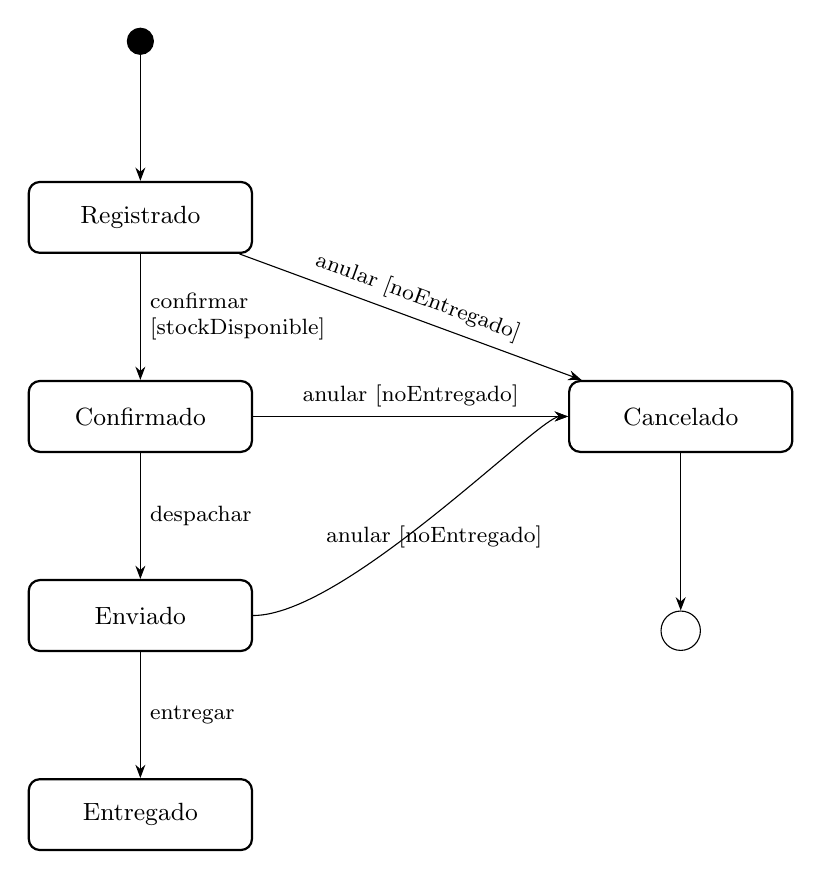
\begin{tikzpicture}[
    node distance=1.6cm and 2.4cm,
    state/.style={rectangle, rounded corners, draw=black, thick, text width=2.6cm, align=center, minimum height=0.9cm, font=\small},
    initial/.style={circle, draw=black, fill=black, minimum size=0.3cm},
    finalring/.style={circle, draw=black, minimum size=0.5cm},
    final/.style={circle, draw=black, fill=black, minimum size=0.3cm},
    >=Stealth
]

\node[initial] (start) {};
\node[state, below=of start] (reg) {Registrado};
\node[state, below=of reg] (conf) {Confirmado};
\node[state, below=of conf] (env) {Enviado};
\node[state, below=of env] (ent) {Entregado};
\node[state, right=4cm of conf] (canc) {Cancelado};
\node[finalring, below=2cm of canc] (endring) {};

\draw[->] (start) -- (reg);
\draw[->] (reg) -- node[right, font=\footnotesize, align=left, text width=3cm] {confirmar\newline{}[stockDisponible]} (conf);
\draw[->] (conf) -- node[right, font=\footnotesize] {despachar} (env);
\draw[->] (env) -- node[right, font=\footnotesize] {entregar} (ent);

\draw[->] (reg) -- node[above, font=\footnotesize, sloped] {anular [noEntregado]} (canc);
\draw[->] (conf) -- node[above, font=\footnotesize] {anular [noEntregado]} (canc);
\draw[->] (env) .. controls +(2.6,0) and +(-1.8,0) .. node[below, font=\footnotesize, pos=0.5] {anular [noEntregado]} (canc);

\draw[->] (canc) -- (endring);

\end{tikzpicture}
\end{center}

\subsection*{Transiciones}

\begin{center}
\small
\begin{tabular}{lllc}
\toprule
\textbf{Estado origen} & \textbf{Evento} & \textbf{Guarda} & \textbf{Estado destino} \\
\midrule
Registrado & confirmar & [stockDisponible] & Confirmado \\
Registrado & notificarFaltante & [stockInsuficiente] & Registrado \\
Confirmado & despachar & --- & Enviado \\
Enviado & entregar & --- & Entregado \\
Registrado & anular & [noEntregado] & Cancelado \\
Confirmado & anular & [noEntregado] & Cancelado \\
Enviado & anular & [noEntregado] & Cancelado \\
\bottomrule
\end{tabular}
\end{center}

La guarda \texttt{[noEntregado]} es importante porque el caso especifica que el pedido puede anularse mientras no haya sido entregado.

% =====================================================
\section{Consistencia entre las tres perspectivas}
% =====================================================

La prueba solicita relacionar cada evento de P3 con la acción de P2 y con la entidad/atributo que modifica en P1. También pide encontrar y corregir una inconsistencia.

\subsection*{Tabla de verificación cruzada}

\begin{center}
\small
\begin{tabular}{lll}
\toprule
\textbf{Evento P3} & \textbf{Acción P2} & \textbf{Clase/atributo P1 afectado} \\
\midrule
Registrar pedido & Registrar pedido & Pedido.fecha, Pedido.total, Pedido.estado \\
Verificar stock & Verificar stock & Producto.stock \\
Confirmar & Confirmar pedido & Pedido.estado \\
Notificar faltante & Notificar faltante & Pedido.estado / notificación \\
Despachar & Enviar pedido & Pedido.estado \\
Entregar & Entregar pedido & Pedido.estado \\
Anular & Anular pedido & Pedido.estado \\
\bottomrule
\end{tabular}
\end{center}

\subsection*{Inconsistencia detectada}

Encontramos una inconsistencia inicial:

En la máquina de estados aparece el evento \emph{Despachar}, pero el diagrama de actividades de ``Registrar pedido'' no contempla la acción de despacho.

\textbf{Defecto:} El evento existe en P3, pero no está representado en P2.

\textbf{Corrección:} Se mantiene P2 como el proceso específico Registrar pedido, pero se documenta que el despacho pertenece a un proceso posterior del sistema.

Por tanto, se agrega la actividad:

\begin{center}
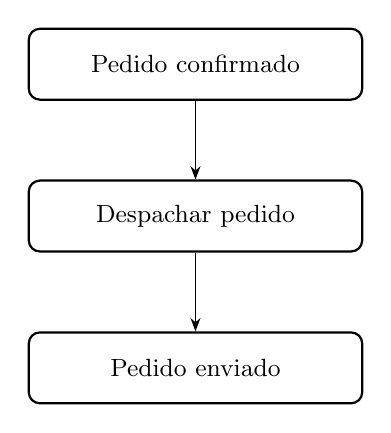
\begin{tikzpicture}[
    node distance=1cm,
    action/.style={rectangle, rounded corners, draw=black, thick, text width=4cm, align=center, minimum height=0.9cm, font=\small},
    >=Stealth
]
\node[action] (a) {Pedido confirmado};
\node[action, below=of a] (b) {Despachar pedido};
\node[action, below=of b] (c) {Pedido enviado};
\draw[->] (a) -- (b);
\draw[->] (b) -- (c);
\end{tikzpicture}
\end{center}

Así queda trazabilidad entre el evento de P3 y una función del sistema.

% =====================================================
\section{Especificación de requisitos}
% =====================================================

La prueba pide exactamente:

\begin{itemize}[nosep]
    \item 2 requisitos funcionales.
    \item 2 no funcionales.
    \item Los no funcionales deben mencionar una característica de ISO/IEC 25010:2023.
    \item Deben tener métrica y umbral.
    \item Todos deben tener identificador, prioridad, estado, fuente, estabilidad, versión y método de verificación.
\end{itemize}

\subsection*{RF-01 --- Registrar pedido}

\textbf{Requisito:} El sistema deberá permitir al cliente registrar un pedido compuesto por una o más líneas de pedido, asociando cada línea con un producto, cantidad y subtotal, y calculando el total del pedido.

\begin{center}
\begin{tabular}{ll}
\toprule
\textbf{Atributo} & \textbf{Valor} \\
\midrule
Identificador & RF-01 \\
Tipo & Funcional \\
Prioridad & Debe \\
Estado & Propuesto \\
Fuente & Caso práctico \\
Estabilidad & Alta \\
Versión & 1.0 \\
Verificación & Prueba funcional \\
\bottomrule
\end{tabular}
\end{center}

\subsection*{RF-02 --- Verificar disponibilidad de stock}

\textbf{Requisito:} El sistema deberá verificar la disponibilidad de stock de los productos antes de confirmar un pedido; si existe stock suficiente, deberá confirmar el pedido y actualizar las existencias, y si no existe, deberá notificar el faltante.

\begin{center}
\begin{tabular}{ll}
\toprule
\textbf{Atributo} & \textbf{Valor} \\
\midrule
Identificador & RF-02 \\
Tipo & Funcional \\
Prioridad & Debe \\
Estado & Propuesto \\
Fuente & Caso práctico \\
Estabilidad & Alta \\
Versión & 1.0 \\
Verificación & Prueba funcional \\
\bottomrule
\end{tabular}
\end{center}

\subsection*{RNF-01 --- Tiempo de respuesta}

\textbf{Requisito:} RNF-01: El sistema deberá cumplir la característica de Eficiencia de desempeño de ISO/IEC 25010:2023, registrando un pedido en un tiempo de respuesta menor o igual a 3 segundos en al menos el 95\% de las operaciones realizadas bajo la carga nominal definida.

\begin{center}
\begin{tabular}{ll}
\toprule
\textbf{Atributo} & \textbf{Valor} \\
\midrule
Identificador & RNF-01 \\
Tipo & No funcional \\
Característica ISO 25010 & Eficiencia de desempeño \\
Métrica & Tiempo de respuesta \\
Umbral & $\leq$ 3 segundos \\
Prioridad & Debería \\
Estado & Propuesto \\
Fuente & Caso práctico \\
Estabilidad & Media \\
Versión & 1.0 \\
Verificación & Prueba de rendimiento \\
\bottomrule
\end{tabular}
\end{center}

\subsection*{RNF-02 --- Protección de datos}

\textbf{Requisito:} RNF-02: El sistema deberá cumplir la característica de Seguridad de ISO/IEC 25010:2023, restringiendo el acceso a los datos personales de los clientes exclusivamente a usuarios autenticados y autorizados, con un 100\% de las solicitudes de acceso no autorizadas rechazadas durante las pruebas de seguridad.

\begin{center}
\begin{tabular}{ll}
\toprule
\textbf{Atributo} & \textbf{Valor} \\
\midrule
Identificador & RNF-02 \\
Tipo & No funcional \\
Característica ISO 25010 & Seguridad \\
Métrica & Solicitudes no autorizadas rechazadas \\
Umbral & 100\% \\
Prioridad & Debe \\
Estado & Propuesto \\
Fuente & Caso práctico \\
Estabilidad & Alta \\
Versión & 1.0 \\
Verificación & Prueba de seguridad \\
\bottomrule
\end{tabular}
\end{center}

La exigencia de utilizar una característica de ISO/IEC 25010, métrica y umbral está expresamente indicada en P5.

% =====================================================
\section{Priorización MoSCoW}
% =====================================================

La clasificación debe utilizar Must, Should, Could y Won't have this time, justificando el valor y la viabilidad.

\begin{center}
\small
\begin{tabular}{p{3.2cm}lp{7.5cm}}
\toprule
\textbf{Requisito} & \textbf{Prioridad} & \textbf{Justificación} \\
\midrule
RF-01 Registrar pedido & Debe & Es la función principal del sistema; sin ella no existe gestión de pedidos. \\
RF-02 Verificar stock & Debe & Es indispensable para evitar confirmar pedidos sin existencias. \\
RNF-01 Tiempo de respuesta & Debería & Es importante para la experiencia del usuario, pero puede optimizarse después de implementar las funciones esenciales. \\
RNF-02 Seguridad & Debe & El sistema maneja datos personales y debe protegerlos. \\
\bottomrule
\end{tabular}
\end{center}

\subsection*{Resultado}

\begin{itemize}[nosep]
    \item \textbf{Obligatorio (Must):} RF-01, RF-02, RNF-02
    \item \textbf{Debería (Should):} RNF-01
    \item \textbf{Podría (Could):} Ninguno
    \item \textbf{No tendrá esta vez (Won't have):} Ninguno
\end{itemize}

Esto cumple con el requisito de tener al menos un Must have.

% =====================================================
\section{Validación por inspección --- ISO/IEC/IEEE 29148}
% =====================================================

La prueba exige separar claramente:

\begin{enumerate}[nosep]
    \item Detección de defectos.
    \item Corrección/retrabajo.
\end{enumerate}

Las propiedades solicitadas son:

\begin{itemize}[nosep]
    \item Sin ambigüedad.
    \item Completo.
    \item Singular.
    \item Verificable.
    \item Verídico.
\end{itemize}

\subsection*{Primera inspección --- defectos}

\begin{center}
\small
\begin{tabular}{lccccc p{3cm}}
\toprule
\textbf{Requisito} & \textbf{Sin amb.} & \textbf{Completo} & \textbf{Singular} & \textbf{Verificable} & \textbf{Verídico} & \textbf{Defecto} \\
\midrule
RF-01 & Sí & Sí & Sí & Sí & Sí & Ninguno \\
RF-02 & No & Sí & No & Sí & Sí & Contiene dos comportamientos: confirmar/actualizar y notificar \\
RNF-01 & Sí & Sí & Sí & Sí & Sí & Ninguno \\
RNF-02 & Sí & Sí & Sí & Sí & Sí & Ninguno \\
\bottomrule
\end{tabular}
\end{center}

\subsection*{Defecto detectado en RF-02}

RF-02 combina dos comportamientos:

\begin{enumerate}[nosep]
    \item Confirmar y actualizar stock.
    \item Notificar faltante.
\end{enumerate}

Por lo tanto, no es completamente singular.

\subsection*{Segundo paso --- Retrabajo}

\textbf{RF-02 corregido (versión intermedia):} El sistema deberá verificar la disponibilidad de stock suficiente para los productos incluidos en un pedido antes de confirmar dicho pedido.

Y se incorpora otro requisito funcional:

\textbf{RF-03:} Cuando el stock disponible no sea suficiente para completar un pedido, el sistema deberá notificar al cliente los productos que presenten faltantes.

Sin embargo, esto nos dejaría con 5 requisitos, mientras que P5 exige exactamente 4.

Por ello, para mantener la estructura solicitada, podemos corregir RF-02 manteniendo cuatro requisitos:

\textbf{RF-02 corregido:} El sistema deberá verificar la disponibilidad de stock de los productos antes de confirmar un pedido y deberá determinar el resultado de la operación como ``stock disponible'' o ``stock insuficiente''.

La notificación queda como acción asociada al resultado del proceso de P2.

\subsection*{Resultado de la segunda inspección}

\begin{center}
\small
\begin{tabular}{lccccc}
\toprule
\textbf{Requisito} & \textbf{Sin ambigüedad} & \textbf{Completo} & \textbf{Singular} & \textbf{Verificable} & \textbf{Verídico} \\
\midrule
RF-01 & Sí & Sí & Sí & Sí & Sí \\
RF-02 corregido & Sí & Sí & Sí & Sí & Sí \\
RNF-01 & Sí & Sí & Sí & Sí & Sí \\
RNF-02 & Sí & Sí & Sí & Sí & Sí \\
\bottomrule
\end{tabular}
\end{center}

\end{document}
